\begin{enumerate}\setcounter{enumi}{2}\bfseries
    \item  \textbf{Apresente um artigo científico recente de uma solução para um problema de Ética em IA.}
\end{enumerate}

O artigo \textit{A Pathway Towards Responsible AI Generated Content} tem como propósito apresentar 
os riscos decorrentes do uso de modelos de geração de conteúdo por Inteligência Artificial (GCIA), 
principalmente aqueles voltados para a produção de conteúdo artístico,
discute e apresenta possíveis ações para o uso responsável, seguro e ético desses modelos na 
sociedade \cite{chen2023pathway}.
Os tipos de conteúdos considerados nesses modelos são bastante variados podendo ser imagens, textos, 
áudios ou vídeos. A maioria dos geradores de textos tem como base GPT
(\textit{Generative Pre-trained Transformers}) e suas versões evoluídas GPT-2 e GPT-3. 
Existe também os geradores de imagens a partir de textos tendo (\textit{text-to-image}) 
como base CLIP e OpenClip. Destaca-se 
recentemente o DALL-E e DALL-E 2 desenvolvidos pela OpenAI, e o Stable Diffusion desenvoldido pela 
Stability DI.

O uso extensivo desses modelos traz preocupações muito relevantes, pois pode afetar a privacidade das pessoas, 
gerar preconceito, informação tóxica, desinformação, provocar desrespeito à propriedade intelectual e 
proporcionar potencial uso indevido quer seja pelas empresas ou pelas pessoas. 

Uma questão relevante surgiu recentemente com a disponibilização de novas funcionalidades no ChatGPT, desenvolvido 
pelo OpenAI, as quais permitem fazer a depuração de código fonte de programas de 
computador ou elaborar trabalhos escolares/acadêmicos. Dependendo da forma como o produto dessas funcionalidades 
for utilizado, surgem riscos potenciais, pois os modelos respondem com dados conforme foram treinados, muitas das 
vezes replicando conteúdos com os quais foram treinados e com sua elavada capacidade de memorização, produzem respostas.
O conjunto de dados utilizados para treinamento frequentemente tem origem e direitos autorais desconhecidos,
muitas das vezes não passam por uma análise de curadoria cuidadosa. 
Além disso, a maioria dos modelos de GCIA decodificadores de textos são treinados com grandes quantidades 
de dados obtidos da internet, os quais podem conter desvios e tendencias (bias) relacionados a temas sociais, podem ser tóxicos, 
e outras limitações inerentes aos grandes modelos de linguagens.

Para que os modelos de GCIA sejam considerados responsáveis, estes devem ter o seguinte escopo: 
privacidade, viés (tendências), toxicidade, desinformação, proteção da propriedade intelectual. 
Adicionalmente, também devem contemplar a capacidade de serem robusto, possibilitar explicações dos resultados,
devem oferecer código fonte aberto, permitir que os autores dos dados deem consentimento para o uso nos modelos, 
dar publicidade aos créditos autorais dos resultados, oferecer compensação aos proprietários dos dados quando 
estes são utilizados nos modelos e, por fim, possibilitar um ambiente amigável para o seu uso.

Considerando o aspecto de privacidade, os modelos generativos de conteúdo permitem uma vulnerabilidade de ataques de privacidade,
devido ao grande volume de dados duplicados nos datasets de treinamento. 
Esse comportamento de replicação tem sido extensivamente estudado nestes modelos e podem levar 
a resultados de imagens como a combinação de fundo e de objetos de imagens reais. Um exemplo desse resultado 
ocorreu com a Stable Diffusion onde a imagem  final era a combinação simples de imagens do dataset de treinamento 
considerando o plano de fundo (\textit{background}) e plano da frente (\textit{foreground}). Devido a isso, 
esses resultados acabam por divulgar imagens particulares de seus autores reais como se fossem 
imagens do próprio modelo, o que é uma consequencia natural da elevada capacidade de memorização pelos modelos ao longo
do treinamento, reproduzindo essas imagens e não criando novas imagens.

As questões de privacidade ainda não possuem solução definitiva, mas ações vem sendo tomadas para minimizar essas consequencias 
danosas. As companhias tem disponibilizado website para fornecer identificação de imagens já treinadas como a 
companhia de arte Spawning AI. 
Outra ação para evitar a duplicação de dados é o uso de técnicas de deduplicação removendo de forma ampla dados
duplicados utilizados em treinamento. Nessa linha segue a companhia OpenAI que reconhece as dificuldades para eliminar 
completamente dados duplicados. 
Outras companhias como Microsoft e Amazon tem adotado medidas para prevenir o compartilhamento de dados sensíveis pelos seus empregados, 
evitando o uso desses dados em futuras versões de modelos de GCIA.
Atualmente as medidas para evitar o vazamento de dados privados são insuficientes e 
ainda faz-se necessário explorar sistemas confiáveis para a detecção de dados duplicados em modelos generativos e uma 
maior investigação no processo de memorização e generalização em sistemas de aprendizado profundo.

Relativo ao aspecto de vieses ou tendencias, geralmente os dados de treinamento 
utilizados nos modelos de Inteligencia Artifical (IA) são obtidos do mundo real,
os quais, sem a intenção, podem reforçar estereótipos indesejáveis, excluir ou marginalizar certos grupos de indivíduos, 
conter dados tóxicos, pode levar à incitação ao ódio ou violência, além de poder ofender indivíduos. 
Um exemplo de dataset que apresenta esse tipo de problema é o LAION, que contém conteúdos relacionados à estereotipagem social,
pornografia, calúnias racistas e violência. Para minimizar esses problemas, o uso de filtros nos dados é uma possibilidade,
contudo eles podem introduzir vieses nos dados de treinamento e, em seguida, propagar esses vieses nos modelos.

Para ilustrar modelos que podem produzir resultados tendenciosos, a Figura \ref{fig:images_of_three_engineers} apresenta 
imagens geradas por meio do comando \textit{prompt} ``\textit{Three engineers running on the grassland}'' 
e o resultado foram indivíduos do sexo masculino, excluindo indivíduos das minorias raciai e
indicando uma ausencia de diversidade de gênero.
Outras estratégias para minimizar esses vieses são o emprego de técnicas de pré-treinamento aplicadas aos dados antes do treinamento do 
modelo e o contínuo treinamento com as informações mais recentes evitando o 
surgimento de lacunas de informação e garantindo que os modelos permaneçam atualizados, relevantes 
e benéficos para a sociedade. Ainda existem oportunidades para investigação mais profunda desses de vieses, de
toxicidade e de desinformação em todo o ciclo de vida de desenvolvimento dos modelos, 
apesar de ser uma tarefa desafiadora.

% Código para centralizar uma figura e posicioná-la "exatamente" no texto
% O opção 'h' posiciona a imagem
% \centering dentro do ambiente figure centraliza
% \begin{figure}[h]
%   \centering 
%   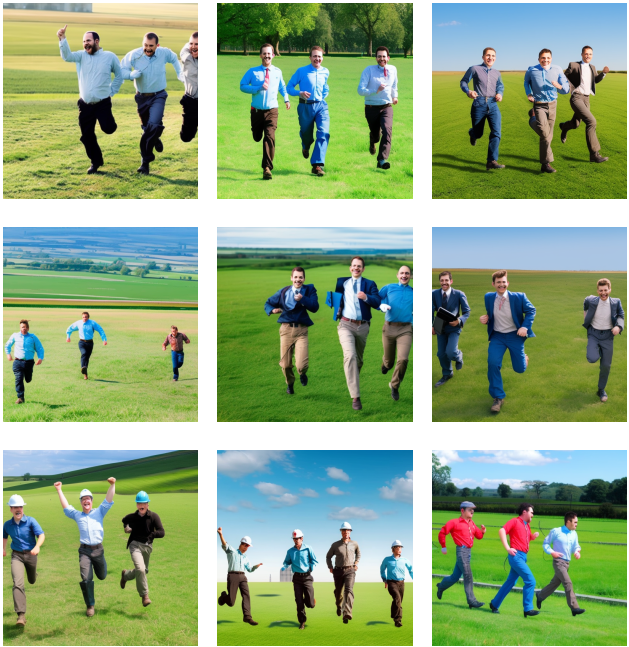
\includegraphics[scale=0.5]{images_generated_with_text_three_engineers.png}
%   \caption{Imagem gerada a partir do texto "Three engineers running on the grassland" by Stable Diffusion v2.1.}
%   \label{fig:images_of_three_engineers}
% \end{figure} 

\begin{wrapfigure}{r}{0.50\textwidth}
  \centering 
  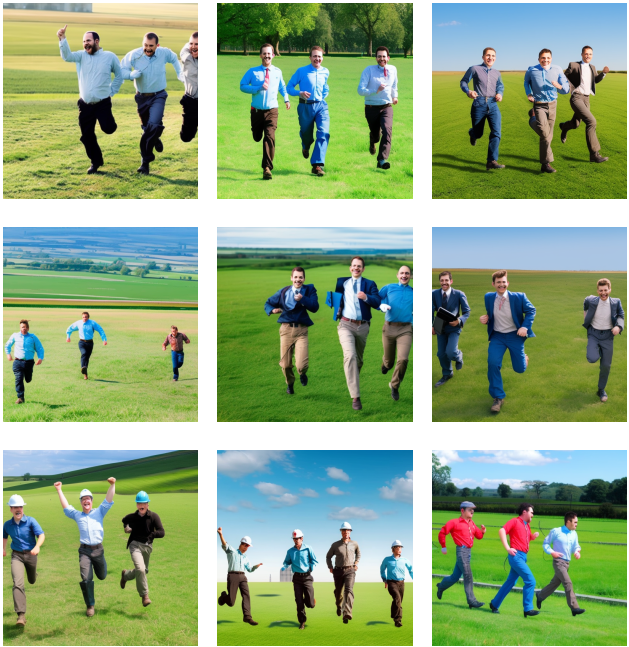
\includegraphics[scale=0.47]{images_generated_with_text_three_engineers.png}
  \caption{Imagem gerada a partir do texto ``Three engineers running on the grassland``  by Stable Diffusion v2.1.}
  \label{fig:images_of_three_engineers}
\end{wrapfigure}


% \begin{wrapfigure}{l}{0.25\textwidth}
%     \centering
%     \includegraphics[width=0.25\textwidth]{contour}
% \end{wrapfigure}

Considerando questões relativas à proteção da propriedade intelectual, 
à medida que as técnicas avançam, surgem situações de violação de direitos autorais
devido os novos conteúdos gerados artificialmente. Um dos desafios nesse aspecto 
é associar a legislação da propriedade intelectual a qual define de forma clara o que é um trabalho original 
e quando o direito à propriedade intelectual é violado. Por isso, a definição de propriedade intelectual no âmbito 
dos modelos de geração de conteúdos por IA ainda permanece obscura e indefinida.
Alguns exemplos de problemas surgem nos modelos generativos 
baseados em texto-para-imagem os quais são acusados de infringir os trabalhos de artistas plástico, 
consequencia do uso de grandes volumes de imagens da internet para o treinamento dos modelos como o Copilot e Stable Diffusion.

Algumas estratégias de minimizar a violação da propriedade intelectual permitem que os artistas solicitem a remoção 
de trabalhos dos datasets que consideram o seu direito violado como a empresa Midjourney. 
Outras companhias como Stability AI planejam permitir que os próprios artistas removam seus trabalhos, 
dando mais flexibilidade ao processo de proteção intelectual. 
Para textos, a marca d'água têm sido utilizada auxiliando na verificação do uso de fontes sem permissão para a geração 
de conteúdos. A companhia OpenAI trabalha para disponibilizar um classificador que consiga diferenciar entre 
texto gerado por modelos de IA de textos escritos por pessoas.


Após breve análise dos principais elementos desejáveis no escopo de GCIA responsáveis, faz-se necessário avaliar  
outras característivas que devem existir nos modelos.

Assim, os conteúdos gerados pelos modelos GCIA podem propagar informação oculta, violenta, danosa e falsa, onde os textos e 
imagens são difíceis de serem diferenciadas de conteúdos criados por pessoas, e podem ser utilizados para propósitos 
de publicação de notícias falsas (\textit{fake news}), boatos e até mensagens de assédio. 
Além disso, o uso para fins comerciais de imagens e textos inseridos 
em produtos e soluções, a integração dos modelos em software e sistemas, a possibiidade da substituição 
de determinados trabalhos realizados por pessoas de uma forma descontrolada gera bastante controversia.

Os modelos podem ser vistos como caixas-preta tendo uma entrada, o processamento que é oculto aos olhos dos usuários 
e a saída, o que leva a uma necessidade de se explicar esse resultado a fim de se compreender como e por quê foi criado.
Adicionalmente a disponibilidade de código-fonte aberto desses modelos pode resultar em riscos de se propagar as falhas 
já mencionadas anteriormente nos novos modelos, produzindo impactos imprevisíveis. 
A possibilidade dos usuários fornecerem devolutivas \textit{feedback} sobre o uso dos modelos é algo necessário
para se ter modelos responsáveis. Como exemplo, a OpenAI possibilita que usuários enviem feedback
os quais são utilizados para a correção e melhoria reduzindo possíveis impactos negativos.

Outro ponto relevante é que os modelos são treinados com dados sem o devido consentimento, desrespeitando os direitos
autorais e sem compensação aos autores pelo uso dos dados. Para evitar esse problema, as companhias passsaram 
a agir de forma ativa junto aos proprietários dos dados antes de realizarem o treinamento de seus modelos. 
Um caminho para contornar essa situação seria as empresas procurarem os autores solicitando autorização 
para uso dos dados bem como recompensá-los quando os dados forem consultados. Com isso haveria uma justa contrapartida 
para os autores e o uso responsável dos dados pelos modelos.

Outros impactos de dimensões menores, contudo não menos importante é o elevado consumo de energia elétrica pelos computadores a fim de treinar os modelos 
cada vez maiores podendo ter bilhões ou trilhões de parâmetros. Isso leva a uma nova reflexão ainda sem uma solução 
concreta. Adicionalmente os modelos deveriam buscar o equilíbrio de benefícios onde determinados grupos de 
pessoas podem ser privilegiadas em detrimento de outros grupos resultando em desigualdades globais.

Por fim, observa-se nos modelos de GCIA a existencia de conflitos entre seus diversos objetivos, pois ao focar na prevenção 
de determinado risco pode-se criar uma vulnerabilidade em outro tipo de risco. Um exemplo seria quando se busca mitigar 
o uso de termos tóxicos em modelos de linguagem podem surgir vieses na predição que discrimina outras 
comunidades.

O artigo finaliza indicando que GCIA ainda está em uma fase embrionária, em crescente e rápida eovlução, 
com tecnologias impressionantes relacionadas ao campo das artes, mas com vários riscos inerentes ao seu uso. 
Fornece um resumo dos atuais e potenciais riscos devido ao uso dos modelos possibilitando que as Companhias
e usuários se previnam, propondo várias ações para minimizar a ocorrência desses riscos.
Conhecê-los, discutí-los, medí-los e agir é um bom caminho para o futuro dos modelos de GCIA responsáveis.
